\chapter{Конструкторская часть}

В данном разделе будут представлены схемы алгоритмов: полного перебора и муравьиного алгоритма. Будут описаны типы и структуры данных, используемые для реализации.

\section{Разработка алгоритмов}

На рисунке \ref{img:brute} приведена схема алгоритма решения задачи коммивояжера полным перебором. Схемы муравьиного алгоритма приведена на рисунке \ref{img:ant}, вспомогательные функции данного алгоритма показаны на рисунках \ref{img:choose}-\ref{img:update}.

\begin{figure}[H]
	\begin{center}
		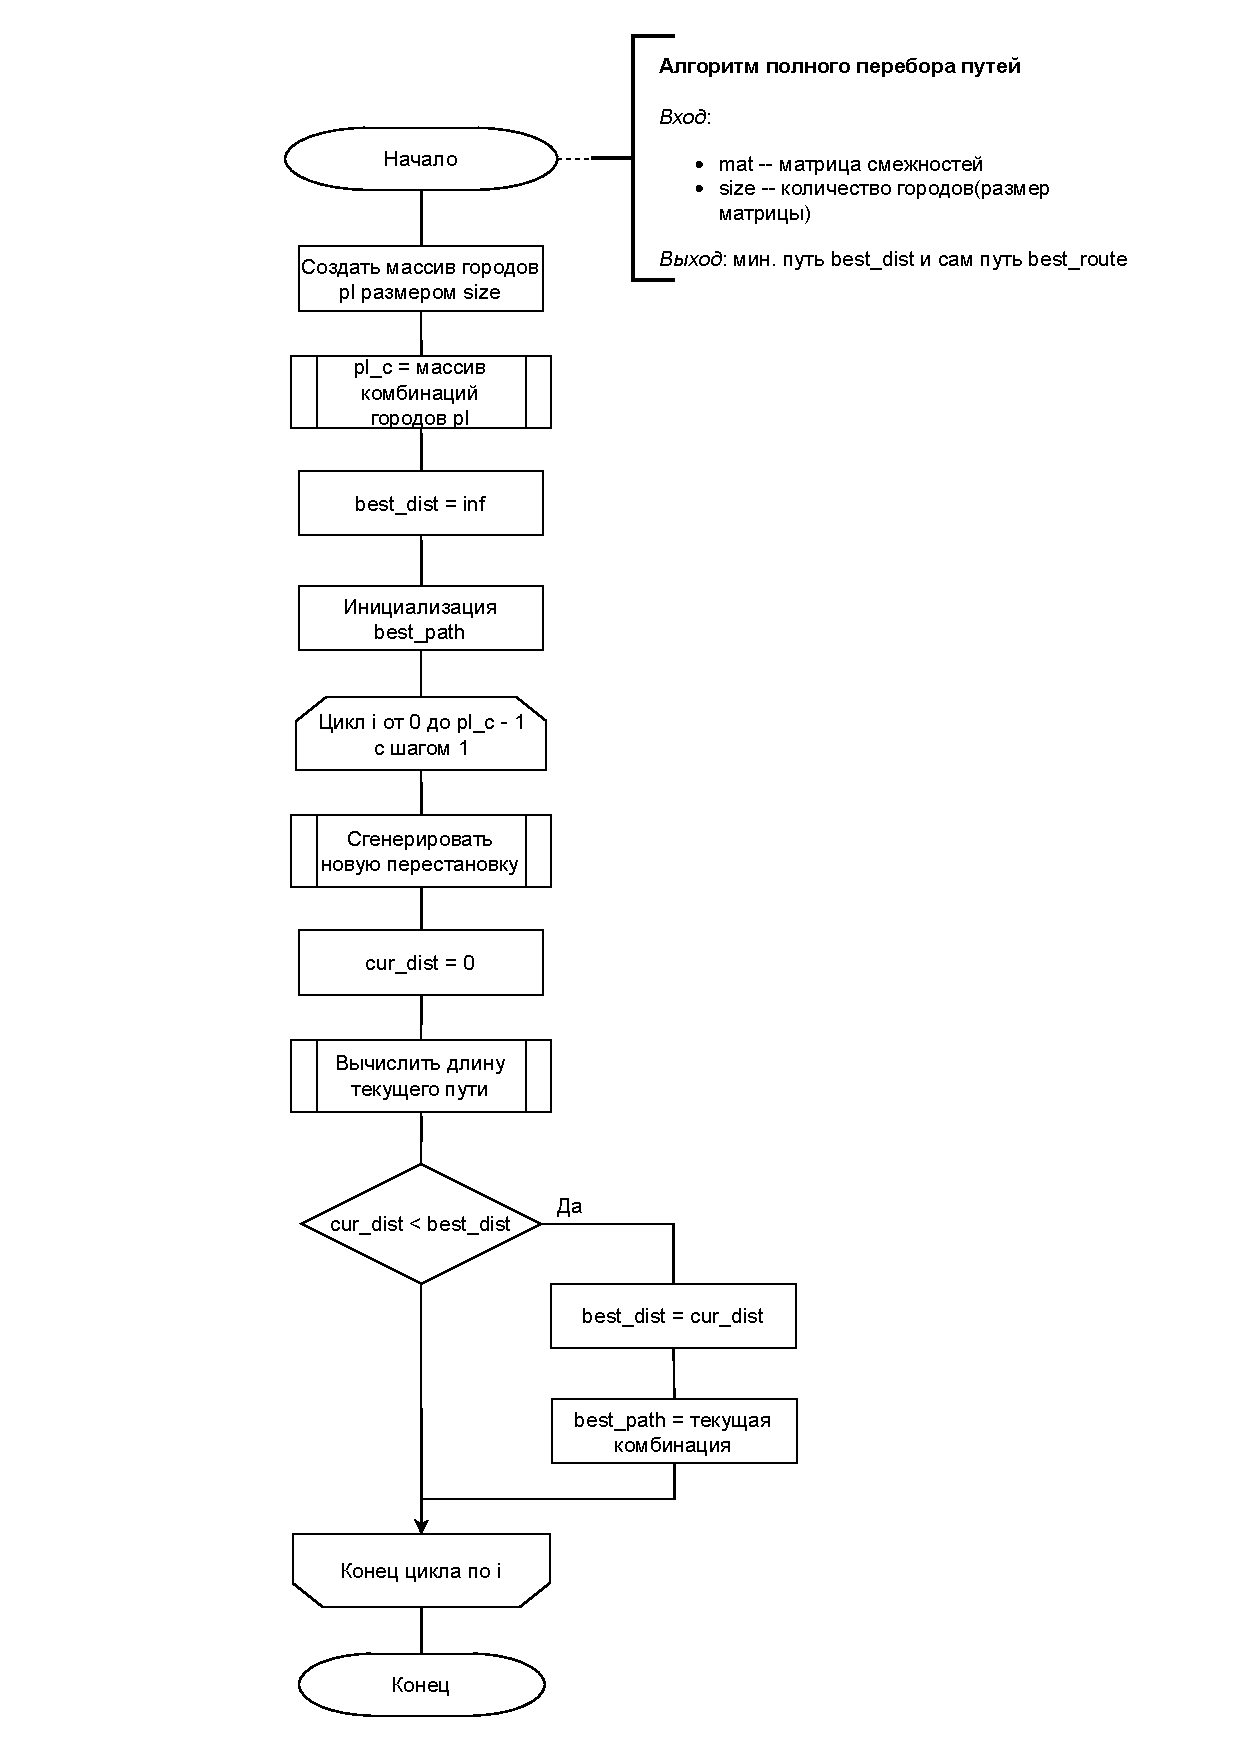
\includegraphics[scale=0.6]{img/brute_force.pdf}
	\end{center}
	\captionsetup{justification=centering}
	\caption{Полный перебор}
	\label{img:brute}
\end{figure}

\begin{figure}[H]
	\begin{center}
		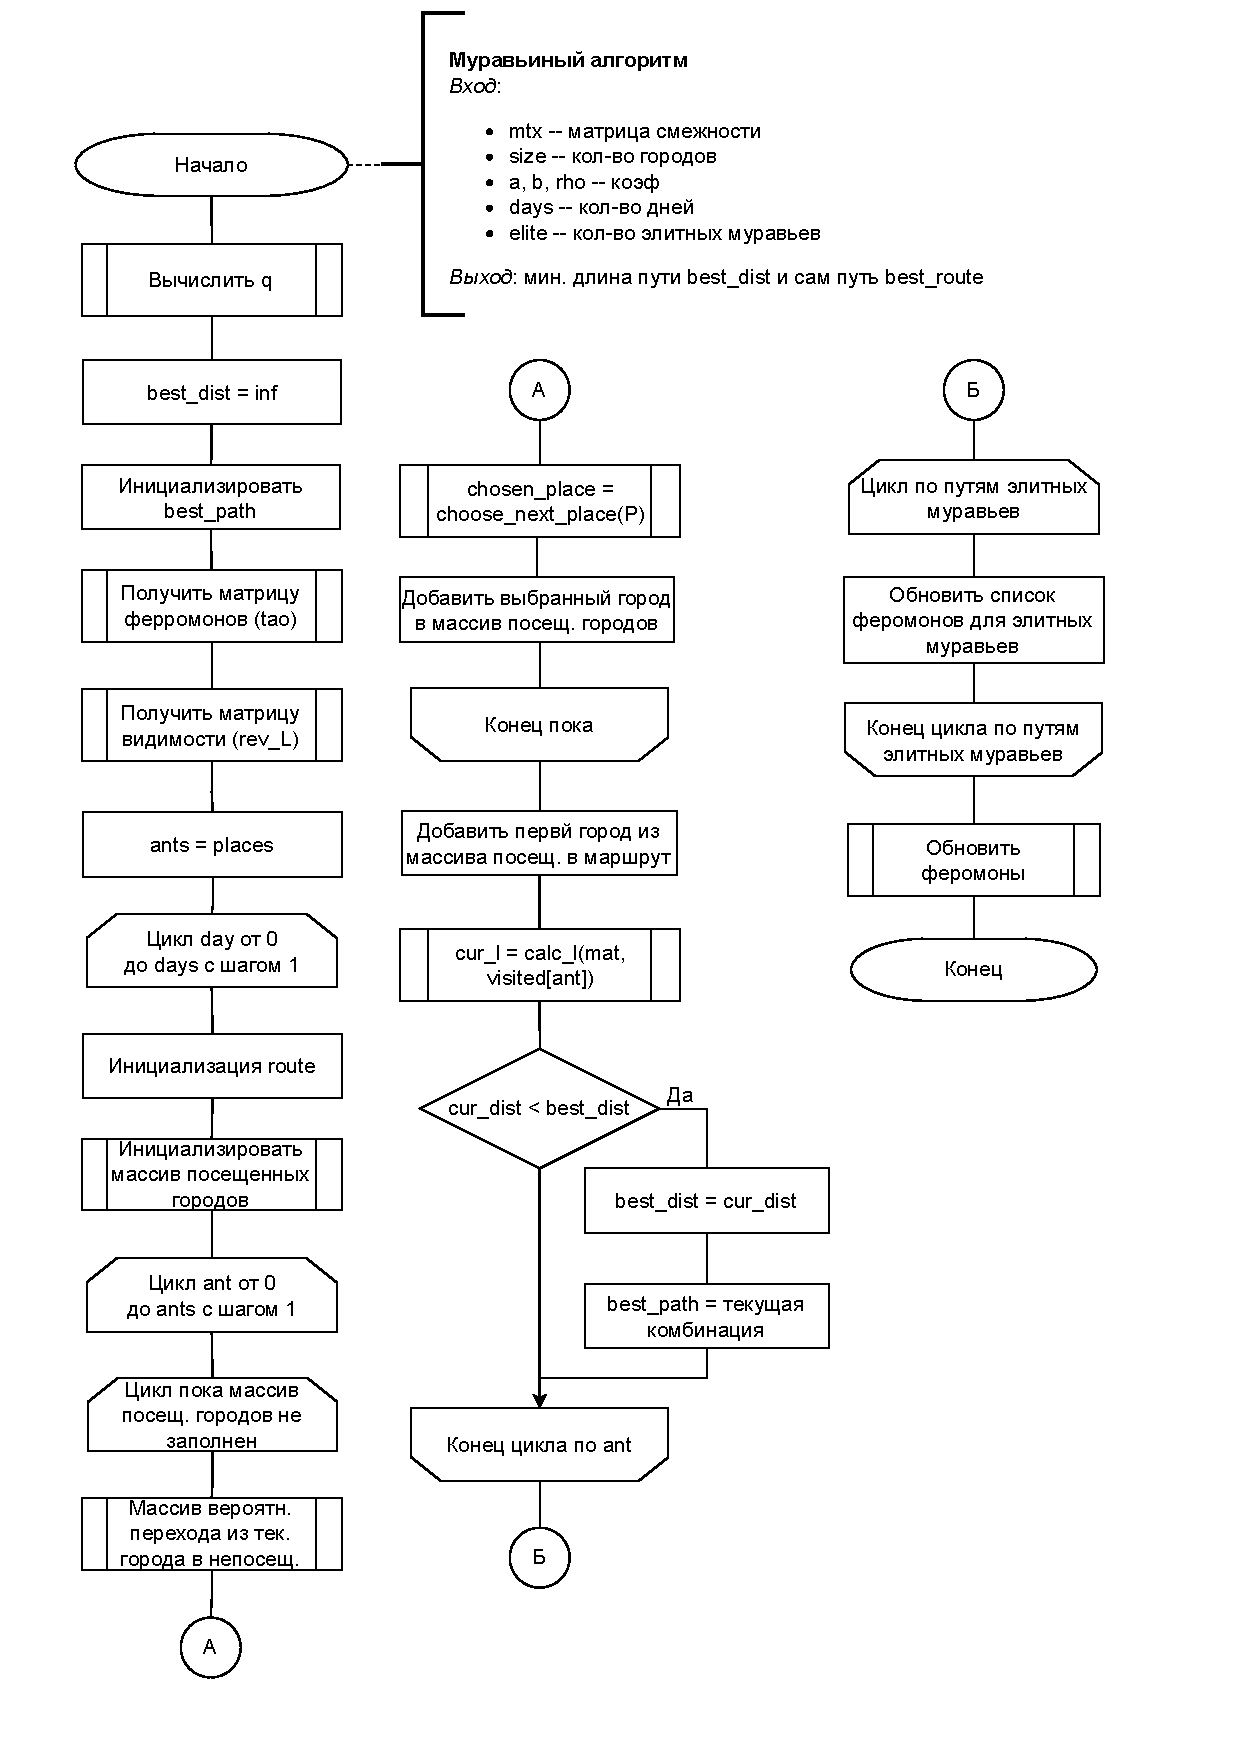
\includegraphics[scale=0.7]{img/ants.pdf}
	\end{center}
	\captionsetup{justification=centering}
	\caption{Муравьиный алгоритм}
	\label{img:ant}
\end{figure}


\begin{figure}[H]
	\begin{center}
		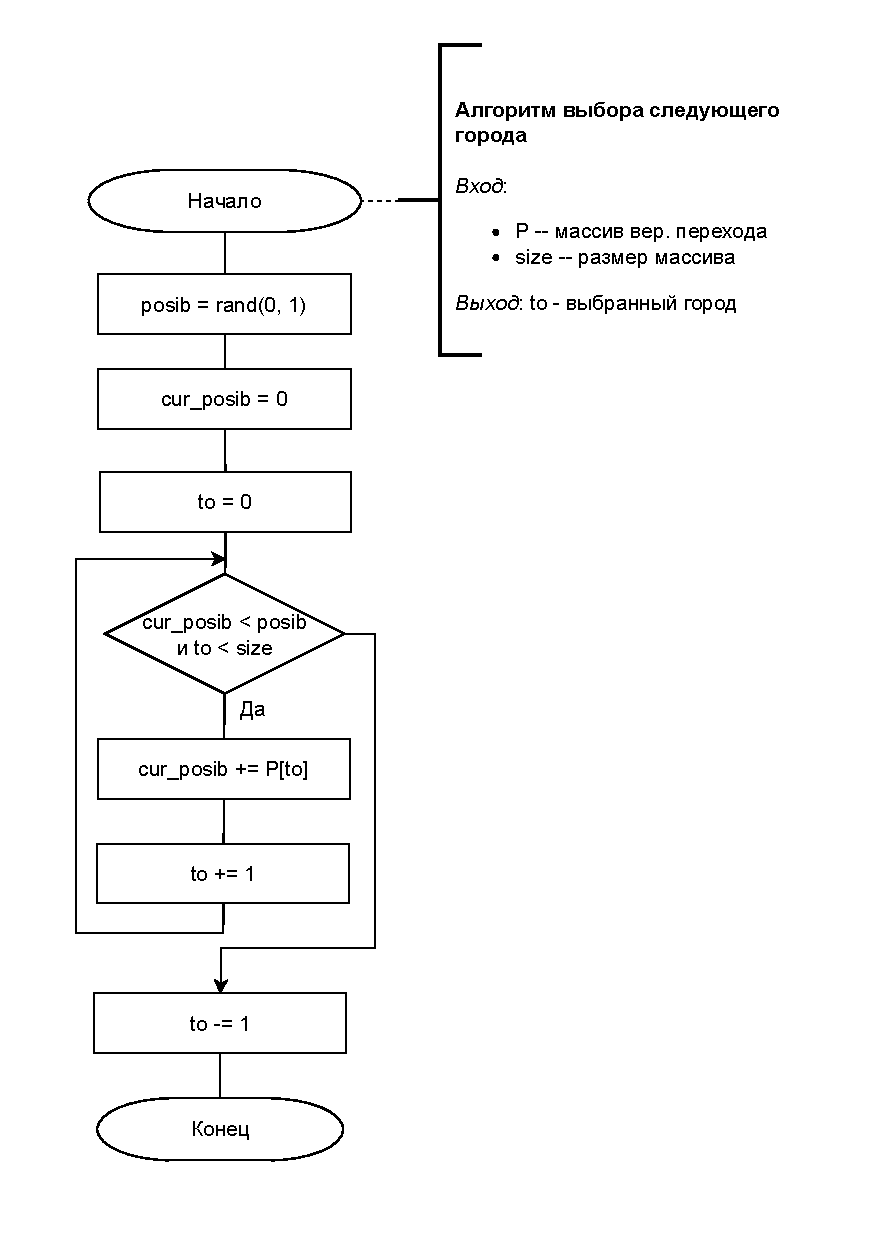
\includegraphics[scale=0.7]{img/cnl.pdf}
	\end{center}
	\captionsetup{justification=centering}
	\caption{Алгоритм выбора следующего города}
	\label{img:choose}
\end{figure}

\begin{figure}[H]
	\begin{center}
		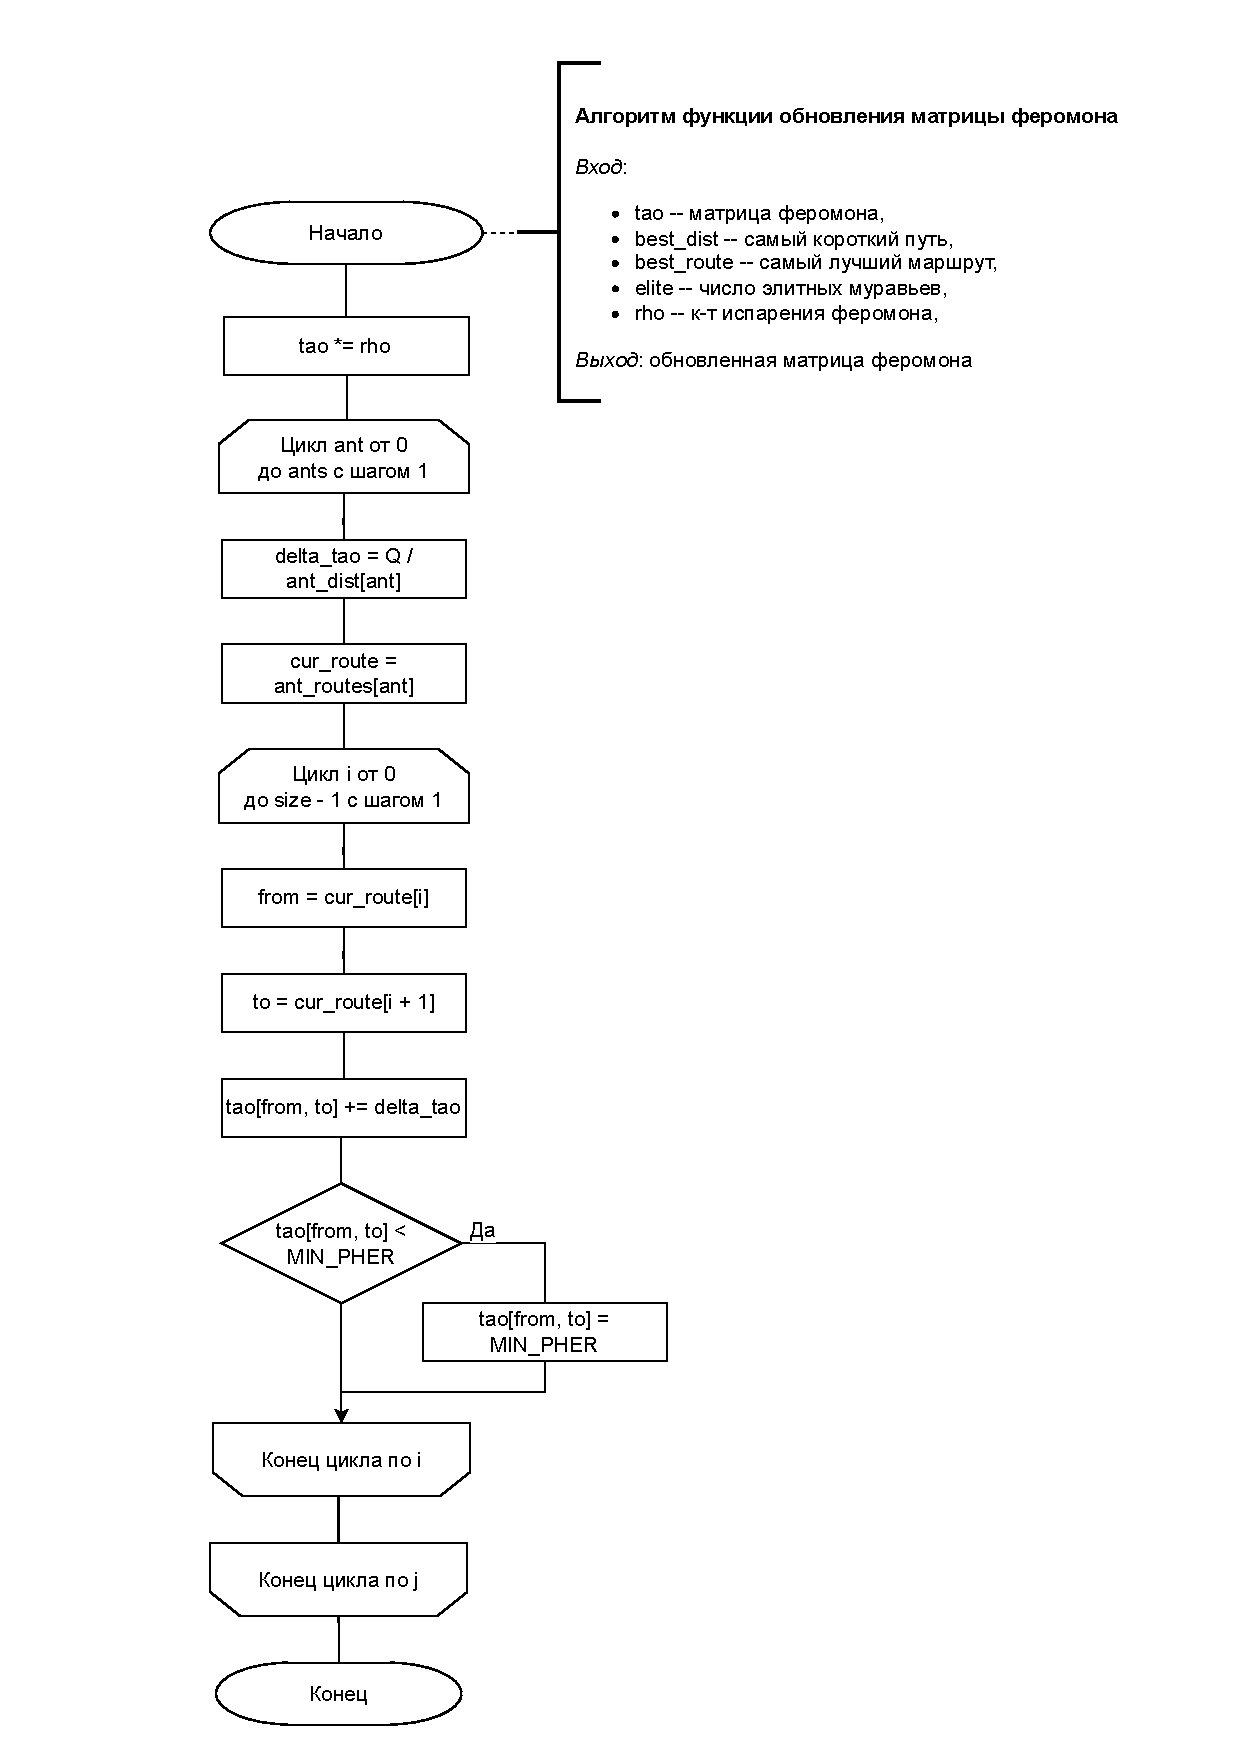
\includegraphics[scale=0.7]{img/up_pher.pdf}
	\end{center}
	\captionsetup{justification=centering}
	\caption{Алгоритм обновления феромона}
	\label{img:update}
\end{figure}

\section{Описание используемых типов и структур данных}

Для задания параметров $\alpha$, $\beta$ и коэффициента $\rho$ - тип данных $float$.

Структура данных - матрица - представляет собой двумерный список значений типа $float$.


\section{Вывод}

Были представлены схемы поиска оптимального пути, проходящего через все города по одному разу. Были указаны типы и структуры данных, используемые для реализации.
